
\medskip


Pour toucher le chapeau d'Averell, Lucky Luke va devoir incliner son pistolet avec précision.

On suppose que les deux cow-boys se tiennent perpendiculairement au sol.

\begin{center}
\begin{tabularx}{0.5\linewidth}{|X|}\hline
Taille d'Avrell : $7$ pieds soit $2,13$ m\\
Distance du sol au pistolet : PS = $1$ m\\
Distance du pistolet à Averell : PA $= 6$ m\\
Le triangle PAC est rectangle en A.\\ \hline
\end{tabularx}
\end{center}

\smallskip

Calculer l'angle d'inclinaison $\widehat{\text{APC}}$ formé par la trajectoire de la balle et l'horizontale. 

Arrondir le résultat au degré près.

\begin{center}
\psset{unit=0.6cm,arrowsize=2pt 4}
\begin{pspicture}(18.5,7)
\rput{15}(16.5,3){\psscalebox{0.32}{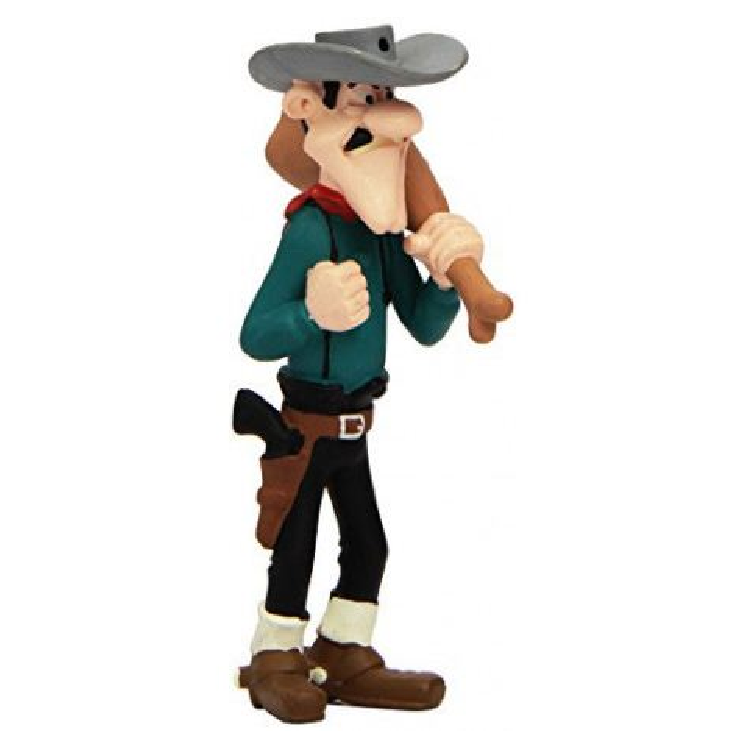
\includegraphics{averell-dalton}}}
\uput[dl](15.4,3){A}\rput{15}(2,2.4){\psscalebox{0.2}{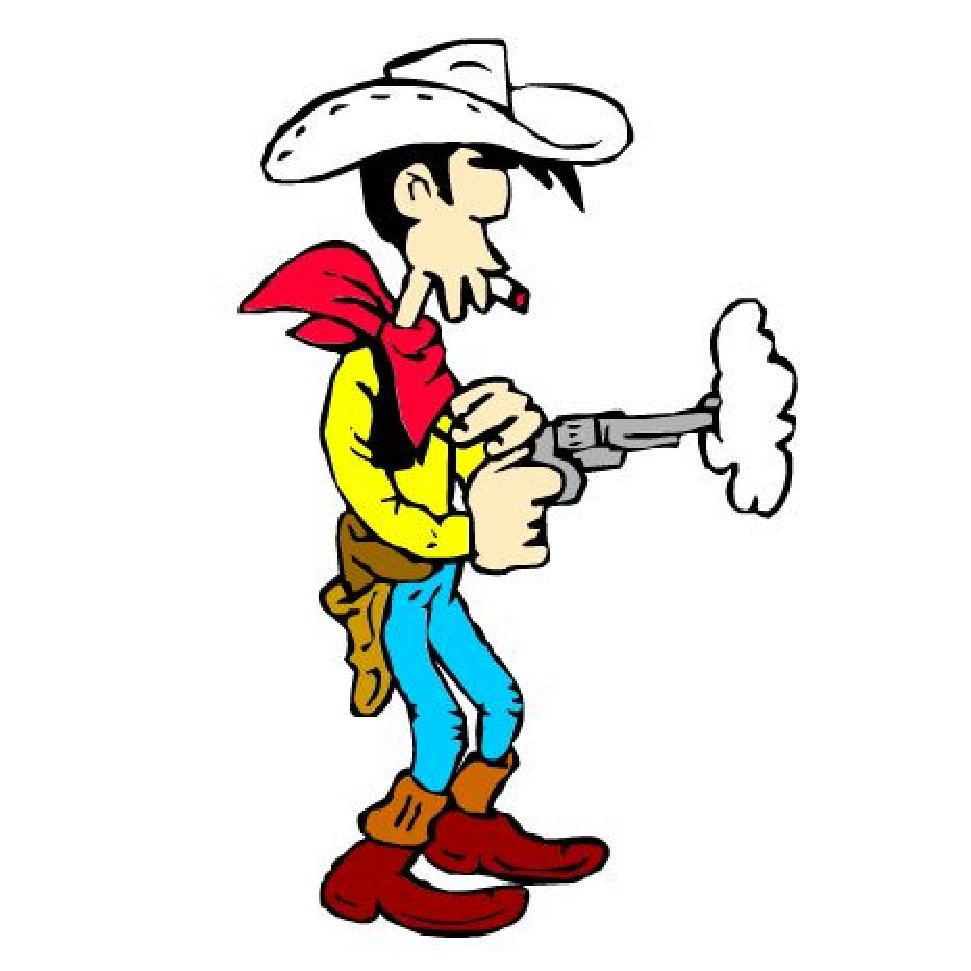
\includegraphics{photo-luky-luke-3}}}
\psline[linewidth=1.5pt](18.5,0)
\pspolygon(2.5,3)(15.9,3)(15.9,6)
\psframe(15.9,3)(15.6,3.3)\psframe(2.5,0)(2.8,0.3)
\psline{->}(2.5,3)(12,5.1)
\psline[linestyle=dashed](2.5,0)(2.5,3)
\rput{12.62}(9.2,4.7){trajectoire de }
\rput{12.62}(9.2,4.3){la balle}
\uput[u](2.5,3){P} \uput[ur](15.9,6){C(hapeau)}

\uput[d](2.5,0){S}
\end{pspicture}
\end{center}

\vspace{0,5cm}

